% Document uses 12 pt font
% 1 in margins
% Contains a relative path for images

\documentclass [10pt]{article}

% page geometry 
\usepackage[margin=1in]{geometry}
\usepackage{changepage}


% ----------  PACKAGES START ------------ %

% Table cell color package and highlighting
\usepackage[table]{xcolor}
\usepackage{color,soul}

% VIC title package
\usepackage{cabin}
\usepackage[T1]{fontenc}

% default font package
%\usepackage{times}
\usepackage{helvet}
%\renewcommand{\familydefault}{\sfdefault}

% ---------- End Font Packages -------------- %

% Title Packages
\usepackage{titlesec}
\usepackage{titletoc}

% Image Package
\usepackage{graphicx}

% Table Packages
\usepackage{longtable}
\usepackage{multirow}
\usepackage{multicol}
\usepackage{multirow}
\usepackage{array}
\renewcommand{\arraystretch}{1.2}% Spread rows out evenly in table
\setlength{\LTpre}{0.5pt} % Reduces white space around tables (top)
%\setlength{\LTpost}{0pt} % Reduces white space around tables (bottom)



% Color Packages
\usepackage{color}   
\definecolor{sectionC}{rgb}{0.016,0.227,.365}
\definecolor{subsectionC}{rgb}{.87,0.87,.87}
\definecolor{subsubsectionC}{rgb}{.94,.93,.90}
\definecolor{tableCell}{rgb}{.96,.95,.90}


% List package
\usepackage{enumitem}
\setenumerate{nosep=0pt, itemindent=0in,leftmargin=.1in, topsep= 2pt,  label = -}


% Paragraph parameter

\setlength{\parindent}{0pt}


% ------------- Creates a linked Table of Contents  Start --------------- %
\usepackage{hyperref}
\hypersetup{
colorlinks=true, %set true if you want colored links
linktoc=all,     %set to all if you want both sections and subsections linked
linkcolor=black,}  %choose some color if you want links to stand out

% ------------- Creates a click-able Table of Contents  End--------------- %

% ---------- PACKAGES END ------------ %



% ------------------- START HEADER AND FOOTER ---------------------------%
\usepackage{fancyhdr}

% Helps with the n of total n pages
\usepackage{lastpage}

\pagestyle{fancy}

% Header
\lhead{Draft Hazard Analysis }
\rhead{Revision: 1}
\fancyhead[LE,CO]{VIC - Group 6}

% Removes line under the header 
\renewcommand{\headrulewidth}{0pt}
\setlength{\headsep}{.2in}

% Footer 

% Set the right side of the footer to be the page number
\fancyfoot[R]{Page \textbf{\thepage}\ of \textbf{\pageref{LastPage}}}
\fancyfoot[C]{}



% ------------------- END HEADER AND FOOTER ---------------------------%

% ------------------- START ROTATE FOOTER ---------------------------%
\usepackage{everypage}


\newcommand{\Lpagenumber}{\ifdim\textwidth=\linewidth\else\bgroup
  \dimendef\margin=0
  \ifodd\value{page}\margin=\oddsidemargin
  \else\margin=\evensidemargin
  \fi
  \raisebox{\dimexpr -\topmargin-\headheight-\headsep-.8\linewidth}[0pt][0pt]{%
    \rlap{\hspace{\dimexpr \margin+\textheight}%
    \llap{\rotatebox{0}{Page \textbf{\thepage}\ of \textbf{\pageref{LastPage}}}}}}%
\egroup\fi}
\AddEverypageHook{\Lpagenumber}%

% ------------------- END ROTATE FOOTER ---------------------------%



% -------- SECTION AND SUBSECTION FORMATING START -------- % 
% starts the 
%\setcounter{section}{1}


\titleformat{\section} % Section
{\normalfont \fontsize{14}{14} \bfseries}{}{0em}{\colorsection}

% Makes a background color
\newcommand{\colorsection}[1]{%
  \colorbox{sectionC}{\parbox{\dimexpr\textwidth-1\fboxsep}{\color{white}\Large\thesection\ \hspace{1mm} #1}}}

% Makes a background color
\titleformat{\subsection} % Subsection
{\normalfont \fontsize{12}{12}  \bfseries}{}{0em}{\colorsubsection }

\newcommand{\colorsubsection}[1]{%
  \colorbox{subsectionC}{\parbox{\dimexpr \textwidth -1\fboxsep}{\large\thesubsection\ #1}}}


% Makes a background color
\titleformat{\subsubsection} % Subsubsection
{\normalfont \fontsize{12}{12} \bfseries}{}{0em}{\colorsubsubsection}

\newcommand{\colorsubsubsection}[1]{%
  \colorbox{subsubsectionC}{\parbox{\dimexpr\textwidth-1\fboxsep}{\thesubsubsection\ #1}}}

% -------- SECTION AND SUBSECTION FORMATING END -------- % 
\usepackage{lipsum}


% -----  IMAGE PATH START -----%
% Relative Image Path
\graphicspath {figures/}
% -----  IMAGE PATH END -----%

% ------ PARAGRAPH FORMAT START ----%
%\setlength{\parskip}{.2em}% Sets the space between new paragraph items 
\setlength{\parindent}{0em} % paragraph indent
% ------ PARAGRAPH FORMAT END ----%


% ------------ BEGIN LANDSCAPE MODE ----------------%
\usepackage{pdflscape}
% ------------ END LANDSCAPE MODE ----------------%


%------------------------------TOC FORMAT START --------------------------------%
\usepackage{tocloft}



% Section indentations
\cftsetindents{section}{0em}{1.5em}
\cftsetindents{subsection}{1em}{2em}
\cftsetindents{subsubsection}{2em}{3em}

% Toc title size
\renewcommand\cfttoctitlefont{\Large\bfseries}
\renewcommand*\contentsname{Table of Contents}

% Removes bold headings from toc
%\renewcommand{\cftsecfont}{\normalfont}

% Removes bold heading page numbers from toc
\renewcommand{\cftsecpagefont}{\normalfont}

% add dots after headings
%\renewcommand{\cftsecleader}{\cftdotfill{\cftdotsep}} 


% number of section headings we want to see in toc
\setcounter{tocdepth}{2}

% Spaceing before headings in toc
\setlength{\cftbeforesecskip}{6pt}

% ------------------------------TOC FORMAT END --------------------------------%








% -------------- DOCUMENT START ---------------%
\begin{document}

% --------- TITLE PAGE START ------- %
\begin {center} 

\thispagestyle{empty}
\vspace*{5cm}

% Logo Insertion
\begin {figure}[h!]
\centering
\hspace{-10mm}
\includegraphics [scale = .5, trim={.4cm 0 .8cm 0},clip] {figures/vic_logo.png}
\end {figure}

{\fontfamily{\cabinfamily}\selectfont
\Huge{Vehicle Intersection Control} }

\vspace{1 cm}
{\Large\textbf{\textsc{McMaster University}}\\}  \vspace {1cm}
{\Large Hazard Analysis\\ \vspace {0.4 cm} SE 4G06}  \vspace {1cm}

{\large \textsc{Group 6} \\} \vspace{1cm}

\begin{tabular}{ l c  l}
Alex Jackson &-& 1302526\\
Jean Lucas Ferreira &-& 1152120 \\
Justin Kapinski &-& 1305257\\
Mathew Hobers &-& 1228607\\
Radhika Sharma &-& 1150430\\
Zachary Bazen &-& 1200979
\end{tabular}




\end{center}

% --------- TITLE PAGE END------- %

\pagebreak

% Inserting table of contents and table of figures 

\tableofcontents
\listoftables
%\listoffigures



\pagebreak

% -----------  REVISION HISTORY START ----------- %

%\section*{Revisions}
%\thispagestyle{empty}
\section{Revisions}
\begin{longtable}{| p{.2\textwidth } | p{.23\textwidth } | p{.21\textwidth } | p{.31\textwidth } |} \caption{VIC Table of Revisions}  \\

\hline 
\centering \textbf{Date} & 
\multicolumn{1}{c}{\textbf {Revision Number}} &
\multicolumn{1}{|c}{\textbf {Authors}} & 
\multicolumn{1}{|c|}{\textbf {Comments}} \\ \hline


\multicolumn{1}{|c|}{\multirow{1}{*}{\centering March 11, 2017}}  & 
\multicolumn{1}{c|}{\multirow{1}{*}{Revision 1}} &
\begin{minipage}{.21\columnwidth} \vspace {1mm}
    Zachary Bazen      \vspace{1mm}
\end{minipage}&
\begin{minipage} {.31\columnwidth}
    \vspace{1mm}\begin{enumerate}[label = - , leftmargin=0.15in]
        \itemsep -.1em
        \item Included acronym, assumptions and safety consideration section
        \item Updated component descriptions 
        \item Updated/improved  information in FMEA worksheet
        \item Added additional details to FMEA worksheet\vspace{1mm}
    \end{enumerate}
\end{minipage}\\ \hline 



\multicolumn{1}{|c|}{\multirow{1}{*}{\centering January 9, 2017}}  & 
\multicolumn{1}{c|}{\multirow{1}{*}{Revision 0}} & 
\begin{minipage}{.21\columnwidth} \vspace {1mm}
    Alex Jackson \newline
    Jean Lucas Ferreira \newline
    Justin Kapinski\newline
    Mathew Hobers\newline
    Radhika Sharma\newline
    Zachary Bazen      \vspace{1mm}
\end{minipage}
&
 \multirow{1}{*}{N/A} \\ 
\hline 


\end{longtable}
% -----------  REVISION HISTORY END ----------- %
\pagebreak

%---------------------------- PROJECT DRIVERS ------------------------%
% heading in document

% -------------- START INTRODUCTION ---------------- %
\section {Introduction}


When multiple autonomous cars arrive at an intersection simultaneously, due to the lack of a decision making protocol, the cars have no way of determining in which order to proceed. The purpose of this project will be create a system that allows autonomous cars to navigate through  intersections. This will be accomplished by providing an appropriate order for the vehicles to proceed through the intersection.  \newline


Vehicle Intersection Control will allow autonomous vehicles to make navigation decisions at intersections. In addition, VIC will be able to dynamically handle changing scenarios at an intersection without running into deadlock or stalemate situations. To ensure safety, VIC will allow cars to navigate through the intersection only after the scheduling algorithm determines the order in which they should proceed. \newline

The following document will outline the hazards that VIC poses to humans, as well hazards to the system. Causes and effect of failures, as well as detection, control and recommended action for failures will also be discussed. 

\section{Acronyms}
\begin{longtable}{|p{.1\textwidth}|p{.3\textwidth}|p{.525\textwidth}|}  \caption{Acronym Definitions and Descriptions } \\ \hline
\rowcolor{subsectionC}\multicolumn{1}{|c|}{\textbf{Acronym}} & \multicolumn{1}{c}{\textbf{Definition}}& \multicolumn{1}{|c|}{\textbf{Description}} \\ \hline
\rowcolor{tableCell}VIC &Vehicle Intersection Control & The name given to the intersection management system\\ \hline
MARC & McMaster Automotive Resource Center & Location of the laboratory used for the project\\ \hline

\end{longtable}



\section{Assumptions}

\begin{longtable}{| p{.2\textwidth } | p{.75\textwidth } | }\hline 
\rowcolor{tableCell}\textbf{HA1} & The risks outlined in the document are poised only to the project stakeholders \\ \hline
\textbf{Rationale} & The project is operating in a restricted access laboratory where only stakeholders are able to gain access  \\ \hline 
\end{longtable}

\begin{longtable}{| p{.2\textwidth } | p{.75\textwidth } | }\hline 
\rowcolor{tableCell}\textbf{HA2} & VIC group members are aware of the risks associated with the VIC system  \\ \hline
\textbf{Rationale} & Ensures the safety of the group members when operating and developing the VIC system  \\ \hline 
\end{longtable}


\begin{longtable}{| p{.2\textwidth } | p{.75\textwidth } | }\hline 
\rowcolor{tableCell}\textbf{HA3} & The risks to humans are low  \\ \hline
\textbf{Rationale} & The VIC system equipment is small and doesn't contain moving parts that could cause significant damage to a human   \\ \hline 
\end{longtable}




\section{Component Descriptions} 
The components can be divided into three parts: vehicle components,  intersection components and communication. The communication component provides means of transferring information between the vehicle components and the intersection components.

\subsection{Vehicle Components}
\subsubsection{Image Processing}
This component allows the vehicle to follow lanes and detect obstacles. It makes use of a WebCam, Raspberry Pi, and algorithms to allow the vehicle to interpret the track environment. 

\subsubsection{Steering Controller}
The steering controller works with the image processing component to steer the vehicle. Further more, the steering controller must make adjustments to ensure the vehicle stays within the track lanes. 

\subsubsection{Speed Controller} 
The speed controller uses a hall effect sensor to determine the speed of the car. This controller will make adjustments to the vehicle's speed according to the track environment.  


\subsection{Intersection Controller}
The intersection camera provides feedback to the intersection controller about approaching vehicles, obstacles in the intersection and departing vehicles. The camera is placed above the intersection and will allow the intersection controller to determine when it is safe for vehicles to proceed through the intersection. 

\subsection{Communication }
The communication component uses Bluetooth communication to facilitate interaction between the vehicle and intersection controller. Vehicles send a request to the intersection controller to proceed through the intersection. When it is safe to proceed the intersection sends back a proceed command. In addition to the proceed command the intersection controller also sends out an emergency stop signal when needed. 









%\subsection{Scheduling Algorithm}

\section{Safety Considerations}

The safety of group and their respective within the MARC laboratory is paramount. Special consideration was taken to determine the risk and failure modes that would impact the those operating within the MARC laboratory. Risks beyond the MARC laboratory are considered outside the scope of the project. Members of the team agree to the hazards associated with the development and operation of the VIC system. Listed bellow are the hazards of the VIC system. 


\subsection{Moving Parts Hazard}

\textbf{Problem}
\begin{enumerate}[label = - , leftmargin=.3in]
        \item Loose/long hair could be caught in moving parts during testing causing a pinching or tearing injury
        \item  Loose clothing could be caught in moving parts during testing\vspace{1mm}
    \end{enumerate}

\textbf{Solution}

\begin{enumerate}[label = - , leftmargin=.3in]
        \item Enclose moving parts where possible
    \end{enumerate}




\subsection{Collision Hazard}
\textbf{Problem}
\begin{enumerate}[label = - , leftmargin=.3in]
        \item Vehicle may leave track and collide with individuals 
        \item Vehicle may leave track and collide with over vehicles 
    \end{enumerate}

\textbf{Solution}

\begin{enumerate}[label = - , leftmargin=.3in]
        \item Ensure individuals stay a safe distance from operating vehicles 
        \item Notify individuals when vehicle operation is about to get underway
        \item Include object detection to prevent collisions
        
    \end{enumerate}


\subsection{Burn Hazard}
\textbf{Problem}
\begin{enumerate}[label = - , leftmargin=.3in]
        \item Vehicle speed controller becomes hot during operation 
    \end{enumerate}

\textbf{Solution}
\begin{enumerate}[label = - , leftmargin=.3in]
        \item Ensure individuals are aware of what the speed controller looks like to prevent accidental contact
        
    \end{enumerate}


\section{FMEA Worksheet}


%\begin{landscape}
%\section{Test}
%Insert Text Here
%
%\end{landscape}




\newpage
\pagestyle{fancy}

\paperwidth=\pdfpageheight
\paperheight=\pdfpagewidth
\pdfpageheight=\paperheight
\pdfpagewidth=\paperwidth
\headwidth=\textheight


\begingroup

%% 
\vsize=\textwidth
\hsize=\textheight



\break
\vspace*{-8.5mm}{
\hspace{-2.1cm}{
    \begin{minipage}{\textwidth}
    


 
 \begin{longtable}{ |p{0.14\textwidth }  | p{0.20\textwidth } |  p{0.22\textwidth } |  p{0.23\textwidth } | p{0.18\textwidth } | p{0.23\textwidth } |  p{0.24\textwidth }|}  \hline

    % ---------------- Block 1------------------- %
    % Row 1
    \rowcolor{subsectionC}\centering \textbf{Design Component} 
    & \multicolumn{1}{c|}{\textbf{Failure Modes} }
    & \multicolumn{1}{c|}{\textbf{Causes of Failure}}
    & \multicolumn{1}{c|}{\textbf{Effects of Failure}}
    & \multicolumn{1}{c|}{\textbf{Detection}} 
    & \multicolumn{1}{c|}{\textbf{Controls} }
    & \multicolumn{1}{c|}{\textbf{ Recommended Action}} \\  \hline
    
    
    
  
        
         % row 8
    \multirow{-1}{*}{\begin{minipage} {.12\columnwidth}
    \begin{center}Intersection \\Camera \end{center}
    \end{minipage}\cellcolor{subsectionC} }
    & \cellcolor{tableCell}\begin{minipage} {.19\columnwidth}
            \begin{center} Failure to detect vehicles \end{center}
        \end{minipage} 
    & \cellcolor{tableCell}\begin{minipage}{.22\textwidth} 
                \vspace {1mm}
                \begin{enumerate}
                    \item Damaged/ disconnected webcam
                    \item Error in software processing image
                    \item Images contain to much noise \vspace {1mm}
                \end{enumerate}
        \end{minipage}
    & \cellcolor{tableCell}\begin{minipage}{.22\textwidth} 
                \vspace{2mm}
                \begin{enumerate}
                    \item Vehicle stalled at intersection
                    \item System deadlock if intersection controller does not detect vehicle leaving 
                    \item Vehicle collision\vspace {1mm}
                \end{enumerate}
        \end{minipage}
    & \cellcolor{tableCell}\begin{minipage}{.18\textwidth} 
                \begin{enumerate}
                    \item Visual inspection of webcam
                    \item Vehicles waiting longer than requirement targets\vspace {1mm}
                \end{enumerate}
        \end{minipage}
    & \cellcolor{tableCell}\begin{minipage}{.22\textwidth} 
                \vspace{2mm}
                \begin{enumerate}
                    \item Bluetooth communication between vehicle and IC \vspace {1mm}
                \end{enumerate}
        \end{minipage}
    
    
    & \cellcolor{tableCell}\begin{minipage}{.24 \columnwidth} 
                \vspace{2mm}
                \begin{enumerate}
                    \item Reconfigure/Replace camera \vspace {1mm}
                \end{enumerate}
        \end{minipage} \\ \hline
        
        
        % Row 6
    \cellcolor{subsectionC}
    &  \begin{minipage} {.19\columnwidth}
            \begin{center} Failure to transmit signal \end{center}
        \end{minipage} 
    & \begin{minipage}{.22\textwidth} 
    
    \vspace {1mm}
                \begin{enumerate}
                    \item Software controlling bluetooth transmitter incorrect
                    \item Damaged transmitter or receiver 
                    \item Loss of power\vspace {1mm}
                \end{enumerate}
        \end{minipage}
    & \begin{minipage}{.22\textwidth} 
                \vspace{2mm}
                \begin{enumerate}
                    \item Vehicle waits too long at intersection
                    \item Vehicle goes through intersection at the wrong time\vspace {1mm}
                \end{enumerate}
        \end{minipage}
    & \begin{minipage}{.18\textwidth} 
                \begin{enumerate}
                    \item Intersection camera will detect car at intersection \vspace {1mm}
                \end{enumerate}
        \end{minipage}
    & 
    
    
    & \begin{minipage}{.24 \columnwidth} 
                \vspace{2mm}
                \begin{enumerate}
                    \item Refresh/Restart communication software
                    \item Vehicle shut down and repair/replace device\vspace {1mm}
                \end{enumerate}
        \end{minipage} \\ \cline{2-7}
    
    % Row 7 
    \multirow{-5}{*}{\begin{minipage} {.12\columnwidth}
    \begin{center} \small Communication \end{center}
    \end{minipage}\cellcolor{subsectionC} }
    & \cellcolor{tableCell}\begin{minipage} {.19\columnwidth}
            \begin{center}Failure to maintain signal \end{center}
        \end{minipage} 
    & \cellcolor{tableCell}\begin{minipage}{.22\textwidth} 
                \begin{enumerate}
                    \item Low signal due to reduced battery power
                    \item Car distance out of range
                    \item Loss of power \vspace {1mm}
                \end{enumerate}
        \end{minipage}
    & \cellcolor{tableCell}\begin{minipage}{.22\textwidth} 
                \vspace{2mm}
                \begin{enumerate}
                    \item Vehicle waits too long at intersection
                    \item Vehicle goes through intersection at the wrong time \vspace {1mm}
                \end{enumerate}
        \end{minipage}
    & \cellcolor{tableCell}\begin{minipage}{.18\textwidth} 
                \begin{enumerate}
                    \item Intersection Sensors will detect car at intersection \vspace {1mm}
                \end{enumerate}
        \end{minipage}
    & \cellcolor{tableCell} 
    
    
    & \cellcolor{tableCell}\begin{minipage}{.24 \columnwidth} 
                \vspace{2mm}
                \begin{enumerate}
                    \item Refresh/Reconnect 
                    \item Vehicle Shut down and repair/replace device\vspace {1mm}
                \end{enumerate}
        \end{minipage} \\ \hline
    
   
    
    
    
      % Row 2
    \cellcolor{subsectionC}
    &  \begin{minipage} {.19\columnwidth}
            \begin{center}Incorrect  Obstacle Detection \end{center}
        \end{minipage} 
    & \begin{minipage}{.22\textwidth} 
        \vspace{1mm}
                \begin{enumerate}
                    \item Webcam physically damage
                    \item Error in software processing image
                    \item Slow feedback due to processing time targets being missed
                    \item Low power or loss of power
                    \item Images contain to much noise\vspace {1mm}
                \end{enumerate}
        \end{minipage}
    & \begin{minipage}{.22\textwidth} 
                \vspace{2mm}
                \begin{enumerate}
                    \item Collision with humans resulting in injury
                    \item Collision with cars and other objects resulting in property damage
                \end{enumerate}
        \end{minipage}
    & \begin{minipage}{.18\textwidth} 
                \begin{enumerate}
                    \item Visual inspection of webcam
                    \item Low battery alert \vspace {1mm}
                \end{enumerate}
        \end{minipage}
    & \begin{minipage}{.22\columnwidth} 
                \vspace{2mm}
                \begin{enumerate}
                    \item Image processing algorithm must respond within a required time
                    \item Ensure track is clear and no undesired objects are present\vspace {1mm}
                \end{enumerate}
        \end{minipage}
    
    
    & \begin{minipage}{.24 \columnwidth} 
                \vspace{2mm}
                \begin{enumerate}
                    \item If too many consecutive deadlines are missed, controller will adjust speed
                    \item EIf RasberryPi battery dies alert the car controller to go in emergency shutdown mode\vspace {1mm}
                \end{enumerate}
        \end{minipage} \\ \cline{2-7}
    
    % Row 3 
    \multirow{-8}{*}{\begin{minipage} {.12\columnwidth}
    \begin{center}Image \\Processing \end{center}
    \end{minipage} \cellcolor{subsectionC} }
    & \cellcolor{tableCell}\begin{minipage} {.19\columnwidth}
            \begin{center}Incorrect  Lane Following \end{center}
        \end{minipage} 
    & \cellcolor{tableCell}\begin{minipage}{.22\columnwidth} 
                \vspace{1mm}
                \begin{enumerate}
                    \item Webcam physically damage
                    \item Images contain to much noise
                    \item Slow feedback due to processing time targets being missed
                    \item Dead battery degrades RasberryPi performance \vspace {1mm}
                \end{enumerate}
        \end{minipage}
    & \cellcolor{tableCell}\begin{minipage}{.22\columnwidth} 
                \vspace{1mm}
                \begin{enumerate}
                    \item Collision with humans resulting in injury
                    \item Collision with cars and other objects resulting in property damage
                    \item Vehicle exits intended lane
                    \item Image proccesing degrades or fails to operate \vspace {1mm}
                \end{enumerate}
        \end{minipage}
    & \cellcolor{tableCell}\begin{minipage}{.18\columnwidth} 
                \begin{enumerate}
                    \item Visual inspection of webcam
                    \item Low battery alert \vspace {1mm}
                \end{enumerate}
        \end{minipage}
    & \cellcolor{tableCell}\begin{minipage}{.23\columnwidth} 
                \vspace{1mm}
                \begin{enumerate}
                    \item Image processing algorithm must respond within a required time
                    \item Ensure track and surrounding area is clear and no undesired objects are present\vspace {1mm}
                \end{enumerate}
        \end{minipage}
    
    
    & \cellcolor{tableCell}\begin{minipage}{.24 \columnwidth} 
                \vspace{1mm}
                \begin{enumerate}
                    \item If too many consecutive deadlines are missed, controller will adjust speed
                    \item EIf RasberryPi battery becomes low alert the car controller to go in emergency shutdown mode\vspace {1mm}
                \end{enumerate}
        \end{minipage} \\ \hline
   
    
   
    
 
    
    
   
    
     
    \end{longtable}
    
    
    
    \end{minipage}}}
    
    
    \break
\vspace{6mm}
\hspace{-2.15cm}{
    \begin{minipage}{\textwidth}
    


 
 \begin{longtable}{ |p{0.14\textwidth }  | p{0.20\textwidth } |  p{0.22\textwidth } |  p{0.23\textwidth } | p{0.18\textwidth } | p{0.22\textwidth } |  p{0.24\textwidth }|}  \hline
 
    
    % ---------------- Block 3------------------- %
    
    % row 5
    \multirow{-1}{*}{\begin{minipage} {.12\columnwidth}
    \begin{center}Speed \\Controller \end{center}
    \end{minipage} \cellcolor{subsectionC} }
    & \cellcolor{tableCell}\begin{minipage} {.19\columnwidth}
            \begin{center}Incorrect  Speed \end{center}
        \end{minipage} 
    & \cellcolor{tableCell}\begin{minipage}{.22\textwidth} 
                \vspace {1mm}
                \begin{enumerate}
                    \item Overheated speed controller degrades performance
                    \item Incorrect speed calculation 
                    \item Hall Effect sensor not working/inaccurate
                    \item Motor failure
                    \item Disconnect wires
                    \item Low power or loss of power\vspace {1mm}
                \end{enumerate}
        \end{minipage}
    & \cellcolor{tableCell}\begin{minipage}{.22\textwidth} 
                \vspace{2mm}
                \begin{enumerate}
                    \item Failure to stop at intersection
                    \item Overshooting lanes when turning
                    \item Vehicle instability 
                    \item Collision with vehicle or cars\vspace {1mm}
                \end{enumerate}
        \end{minipage}
    & \cellcolor{tableCell}\begin{minipage}{.18\textwidth} 
                \begin{enumerate}
                    \item Hall Effect sensor
                    \item Visual check \vspace {1mm}
                \end{enumerate}
        \end{minipage}
    & \cellcolor{tableCell}\begin{minipage}{.22\textwidth} 
                \vspace{2mm}
                \begin{enumerate}
                    \item Feedback loop between speed sensor and speed controller \vspace {1mm}
                \end{enumerate}
        \end{minipage}
    
    
    & \cellcolor{tableCell}\begin{minipage}{.24 \columnwidth} 
                \vspace{2mm}
                \begin{enumerate}
                    \item Speed corrected with software
                    \item Vehicle shutdown 
                    \item Recalibrate/Repair/ Replace Speed sensors and/or speed controller \vspace {1mm}
                \end{enumerate}
        \end{minipage} \\ \hline
   
  % ---------------- Block 4------------------- %
  
  
  
     % row 4
    \multirow{-1}{*}{\begin{minipage} {.12\columnwidth}
    \begin{center}Steering  \\Controller \end{center}
    \end{minipage}\cellcolor{subsectionC} \cellcolor{subsectionC}}
    & \begin{minipage} {.19\columnwidth}
            \begin{center}Incorrect  Steering \end{center}
        \end{minipage} 
    & \begin{minipage}{.22\textwidth} 
                \vspace {1mm}
                \begin{enumerate}
                    \item Error is software processing speed 
                    \item Damaged servo operates in unintended fashion
                    \item Disconnected Wires
                    \item Loose steering assembly
                    \item Low power or loss of power\vspace {1mm}
                \end{enumerate}
        \end{minipage}
    & \begin{minipage}{.22\textwidth} 
                \vspace{2mm}
                \begin{enumerate}
                   \item Collision with humans resulting in injury
                    \item Collision with cars and other objects resulting in property damage
                    \item Vehicle Exits Track 
                    \item Vehicle fails to make turn \vspace {1mm}
                \end{enumerate}
        \end{minipage}
    & \begin{minipage}{.18\textwidth} 
                \begin{enumerate}
                    \item Visual inspection of vehicle \vspace {1mm}
                \end{enumerate}
        \end{minipage}
    & \begin{minipage}{.22\textwidth} 
                \vspace{2mm}
                \begin{enumerate}
                    \item Software processing track images \vspace {1mm}
                \end{enumerate}
        \end{minipage}
    
    
    & \begin{minipage}{.24 \columnwidth} 
                \vspace{2mm}
                \begin{enumerate}
                    \item Direction corrected with software
                    \item Shutdown vehicle if servo performance degrades
                    \item Recalibrate/Repair/ Replace Servo \vspace {1mm}
                \end{enumerate}
        \end{minipage} \\ \hline
   
    
    
    
    % ---------------- Block 5------------------- %
   
 
    
    
    
    % ---------------- Block 5------------------- %
 
 
 \end{longtable}
    
    
    
    \end{minipage}}

% \pagebreak

% \begin {figure}[h!]
% %[scale = .5, trim={.4cm 0 .8cm 0},clip] 
% \vspace*{-1.6cm}
% \hspace{-2.3cm}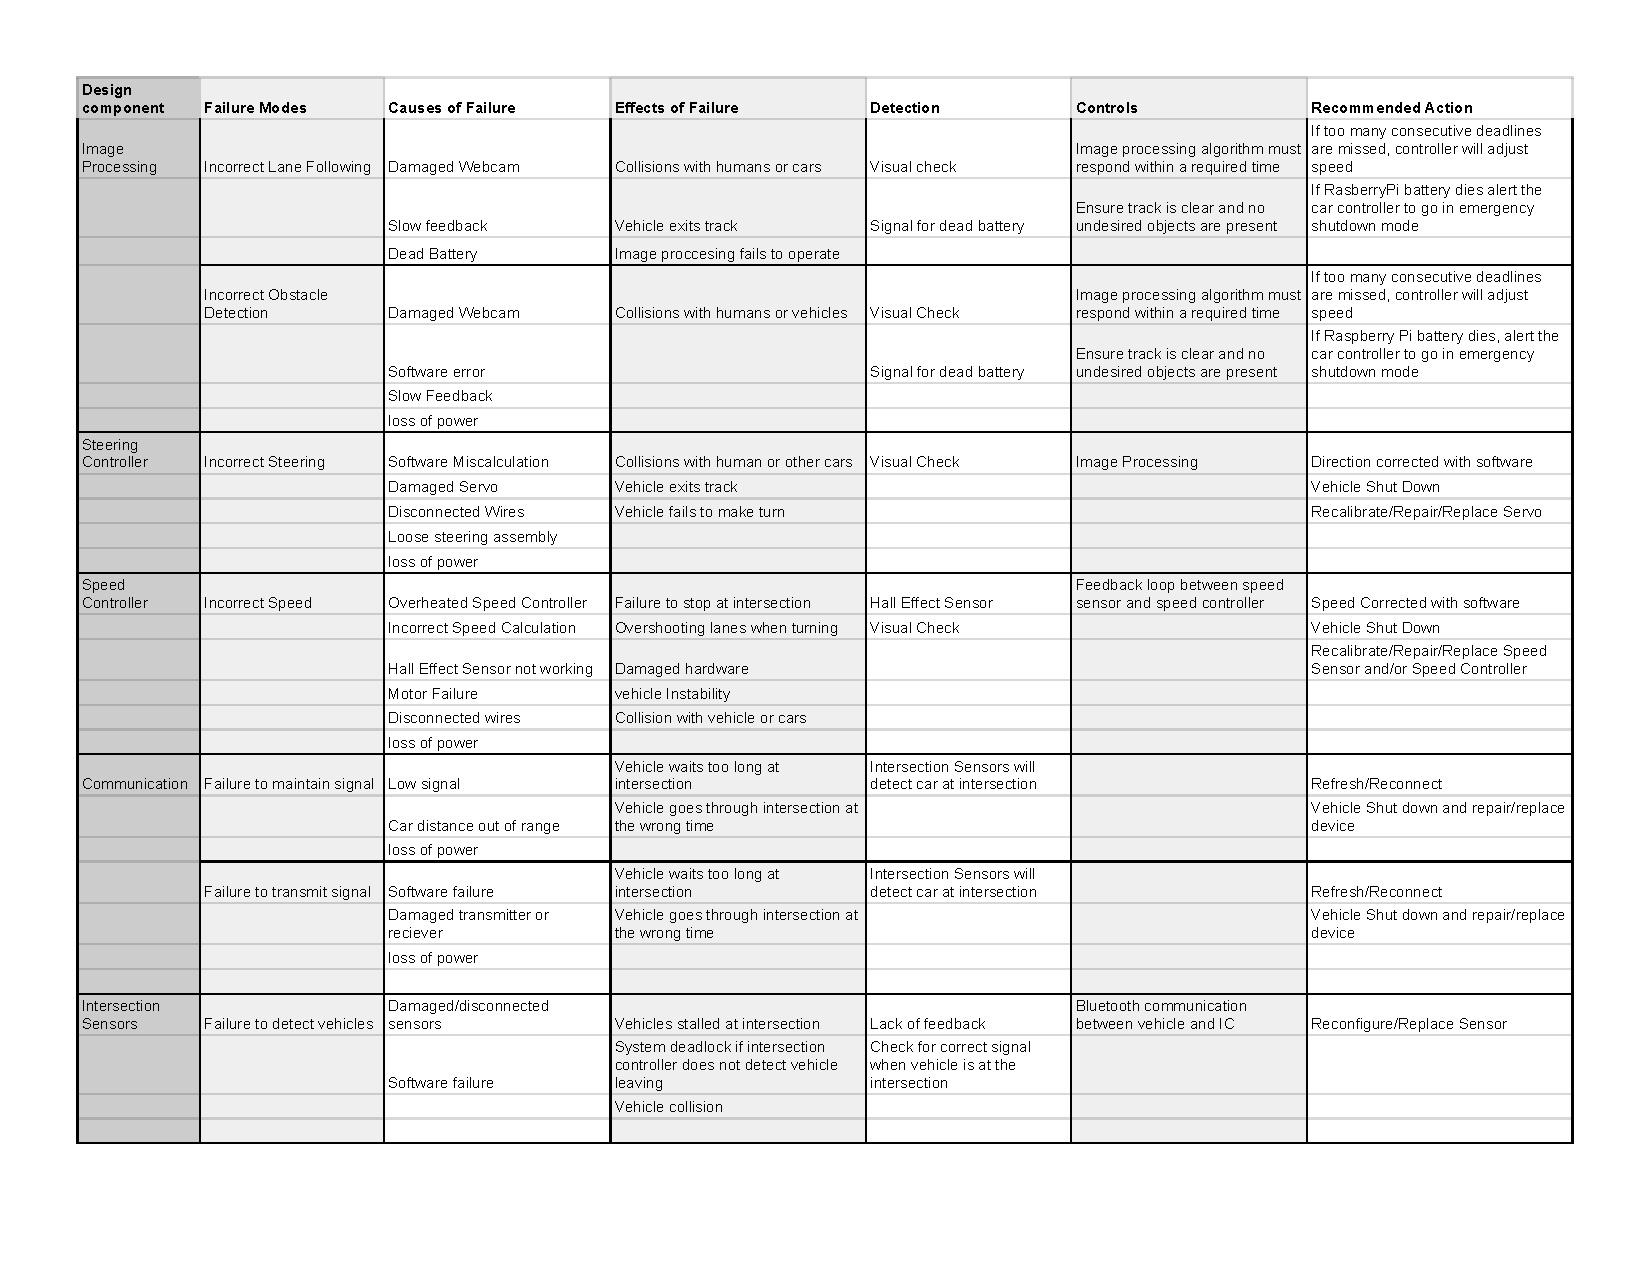
\includegraphics {figures/vic_haz.pdf}

% \end {figure}


% This adds the pagenumber to the rotated page
\begin{landscape}
\end{landscape}
\endgroup


% This resets geometry after the landscape page
\newpage
\paperwidth=\pdfpageheight
\paperheight=\pdfpagewidth
\pdfpageheight=\paperheight
\pdfpagewidth=\paperwidth
\headwidth=\textwidth


\end{document}
